\documentclass[a4paper]{article}
%%\documentclass{amsart}

%% Language and font encodings
\usepackage[english]{babel}
\usepackage[utf8x]{inputenc}
\usepackage[T1]{fontenc}


%% Sets page size and margins
\usepackage[a4paper,top=3cm,bottom=2cm,left=3cm,right=3cm,marginparwidth=1.75cm]{geometry}

%% Useful packages
\usepackage{amsmath}
\usepackage{graphicx}
\usepackage[colorinlistoftodos]{todonotes}
\usepackage[colorlinks=true, allcolors=blue]{hyperref}
\usepackage{listings}
\usepackage{amsfonts}
\usepackage{tikz}
\usepackage{subcaption}
\usepackage{float}
\usepackage{multicol}
\usepackage{lipsum}
\usepackage{mwe}

\usepackage{algorithm}
\usepackage[noend]{algpseudocode}

 \usepackage[usenames,dvipsnames]{pstricks}
 \usepackage{epsfig}
 \usepackage{pst-grad} % For gradients
 \usepackage{pst-plot} % For axes
 \usepackage[space]{grffile} % For spaces in paths
 \usepackage{etoolbox} % For spaces in paths
 \makeatletter % For spaces in paths
 \patchcmd\Gread@eps{\@inputcheck#1 }{\@inputcheck"#1"\relax}{}{}
 \makeatother
 

%\newcommand{\norm}[1]{\left\lVert#1\right\rVert}
\newcommand{\norm}[1]{{\left\vert\kern-0.25ex\left\vert\kern-0.25ex\left\vert #1 
    \right\vert\kern-0.25ex\right\vert\kern-0.25ex\right\vert}}
\newcommand{\vecnorm}[1]{\left\lVert#1\right\rVert}
\newcommand{\trace}[1]{\text{trace}(#1)}
\newcommand{\rank}[1]{\text{rank}(#1)}


\newtheorem{theorem}{Theorem}[section]
\newtheorem{lemma}[theorem]{Lemma}
\newtheorem{remark}[theorem]{Remark}
\newtheorem{corollary}[theorem]{Corollary}
\newtheorem{definition}[theorem]{Definition}

\title{Low Rank Matrix Approximation and Applications}
\author{Math 4370\\ \\ Tyler Evans}

\begin{document}
\maketitle

\begin{abstract}
Representing higher dimensional data in a lower dimensional space can have many benefits.  This paper presents how such a concept can be realized through use of the Eckart-Young Theorem, and presents applications in image compression and classification.
\end{abstract}

\section{Introduction}

Storing as much information as possible is not always a good idea, doing so may result in redundancies or lead to model over-fitting.  A common practice is to employ a reduced rank model in which the high dimensional data is approximated in a lower dimension.

Formalizing this concept, we arrive at the matrix approximation problem: Given a matrix $A$ with rank $r$, what is the best approximation $A_k$ of rank $k$ with $k<r$?  It will be shown how the singular value decomposition leads to an intuitive low rank matrix approximation, and that this is in fact the optimal approximation.

Finally, it will be shown how this technique can be applied directly to image compression as well as developing a reduced rank image classification model.

\section{Theory}

Recall the singular value decomposition (SVD) matrix factorization, presented below with notation consistent with \cite{elden}.  Due to the nature of the applications, we will restrict ourselves to real matrices for simplification.

\begin{theorem}[Singular Value Decomposition]
Suppose that $A\in \mathbb{R}^{m\times n}$ with rank equal to $r$.  Then we can write $A$ as
\begin{equation}
A=U\Sigma V^T
\end{equation}
where $U\in \mathbb{R}^{m\times m}$ and $V\in \mathbb{R}^{n\times n}$ are orthogonal matrices, $\Sigma \in \mathbb{R}^{m\times n}$ with $\sigma_{i,j} = 0$ whenever $i\neq j$, and the main diagonal elements $\sigma_1 \geq \sigma_2 \geq \dots \geq \sigma_r > 0$, $0=\sigma_{r+1} = \dots = \sigma_q$ where $q=\min\{m,n\}$.
\end{theorem}





\subsection{Slim Singular Value Decomposition}

Observe that immediately, the sizes of the matrices that make up the SVD of $A$ can be reduced due to the region of zeros present in $\Sigma$. Illustrated below is a diagram of this effect for the case that $m>n$, in the other case, simply consider $A^T$.
\newcommand{\bigzero}{\mbox{\normalfont\Large 0}}

%\begingroup\makeatletter\def\f@size{5}\check@mathfonts
\begin{center}
\scalebox{0.8}{
$
U \Sigma V^T = 
\begin{bmatrix}
    u_{11} & \dots  & u_{1m} \\
    \vdots & \ddots & \vdots \\
    u_{m1} & \dots  & u_{mm}
\end{bmatrix}
%\underbrace{
\begin{bmatrix}
    \sigma_1 & 0 & \dots  & 0 \\
    0 & \ddots & \ddots & \vdots\\
    \vdots & \ddots & \ddots & 0\\
    0 & \hdots & 0 & \sigma_n\\
    \hline
    0 & \hdots & \hdots & 0\\
    \vdots & \vdots & \vdots & \vdots\\
    0 & \hdots & \hdots & 0
\end{bmatrix}
%}_{m \times n}
\begin{bmatrix}
    v^T_{11} & \dots  & v^T_{1n} \\
    \vdots & \ddots & \vdots \\
    v^T_{n1} & \dots  & v^T_{nn}
\end{bmatrix}
=
\begin{bmatrix}
    u_{11} & \dots  & u_{1n} \\
    \vdots & \ddots & \vdots \\
    u_{m1} & \dots  & u_{mn}
\end{bmatrix}
\begin{bmatrix}
    \sigma_1 & 0 & \dots  & 0 \\
    0 & \ddots & \ddots & \vdots\\
    \vdots & \ddots & \ddots & 0\\
    0 & \hdots & 0 & \sigma_n\\
\end{bmatrix}
\begin{bmatrix}
    v^T_{11} & \dots  & v^T_{1n} \\
    \vdots & \ddots & \vdots \\
    v^T_{n1} & \dots  & v^T_{nn}
\end{bmatrix}
$
}
\end{center}
%\endgroup

We see that the zero region of $\Sigma$ effectively deletes the rightmost columns of $U$.  Now consider what happens when $A$ is not of full rank, that is $A$ has rank $r<\min\{m,n\}$.  We will then have that $\sigma$'s with index larger than $r$ will be zero, which will reduce the effective size of $\Sigma$ even more.  This will result in less columns for $U$ as well as less rows for $V$.

\begin{definition}
When talking about a matrix $A\in \mathbb{R}^{m\times n}$ with SVD $A=U\Sigma V^T$, for $1\leq k$ define:
\begin{enumerate}
\item $U_k \in \mathbb{R}^{m\times k}$ to be the first $m$ rows and $k$ columns of $U$
\item $\Sigma_k \in \mathbb{R}^{k\times k}$ to be the first $k$ rows and $k$ columns of $\Sigma$
\item $V^T_k \in \mathbb{R}^{k\times n}$ to be the first $k$ rows and $n$ columns of $V^T$
\end{enumerate}
\end{definition}

$$
$$

This definition along with the following partitioning can formalize the slim SVD presented above. Consider $A$ of rank $r$:

% and define for any $1\leq k \leq r$:


$$
A = U\Sigma V^T =
\begin{bmatrix}
U_r & U_x\\
\end{bmatrix}
\begin{bmatrix}
\Sigma_r & 0\\
0 & 0
\end{bmatrix}
\begin{bmatrix}
V_r^T \\ V_x^T
\end{bmatrix}
=
U_r \Sigma_r V_r^T
$$
where $U_x$ and $V_x$ are what is left over after partitioning with $U_r$ and $V_r$.  Thus, we see that the rank of $A$ can affect how much of the SVD is relevant.

$$
$$

The concept of the slim SVD can lead us to an important form of the matrix $A$, the outer product form:

%$$
%\text{where} \:
%U_k \in \mathbb{R}^{m\times k}, \: 
%\Sigma_k \in \mathbb{R}^{k\times k}, \:
%V^T_k \in \mathbb{R}^{n\times k}
%$$


%From this point onwards, when we refer to %$U_k,\Sigma_k, V^T_k$ of $A$, we will use their %definition above.


% condensed form which will also lead to outer product derivation!

%$$
%U_s \Sigma_s V^T = 
%\begin{bmatrix}
%u_1 & \dots & u_n
%\end{bmatrix}
%\begin{bmatrix}
%\sigma_1 e_1 & \dots & \sigma_n e_n
%\end{bmatrix}
%\begin{bmatrix}
%v_1^T\\ \vdots \\ v_n^T
%\end{bmatrix}
%=
%\begin{bmatrix}
%u_1 & \dots & u_n
%\end{bmatrix}
%\begin{bmatrix}
%\sigma_1 v_1^T\\ \vdots \\ \sigma_n v_n^T
%\end{bmatrix}
%=
%\sum_{i=1}^n \sigma_i u_i v_i^T
%$$

$$
U_r \Sigma_r V_r^T = 
\begin{bmatrix}
u_1 & \dots & u_r
\end{bmatrix}
\begin{bmatrix}
    \sigma_1 & 0 & \dots  & 0 \\
    0 & \ddots & \ddots & \vdots\\
    \vdots & \ddots & \ddots & 0\\
    0 & \hdots & 0 & \sigma_r\\
\end{bmatrix}
\begin{bmatrix}
v_1^T\\ \vdots \\ v_r^T
\end{bmatrix}
=
\begin{bmatrix}
u_1 & \dots & u_r
\end{bmatrix}
\begin{bmatrix}
\sigma_1 v_1^T\\ \vdots \\ \sigma_r v_r^T
\end{bmatrix}
=
\sum_{i=1}^r \sigma_i u_i v_i^T
$$

$$
$$

This is interesting because it shows how any matrix can be written as a sum of rank 1 matrices.  Furthermore, this form also leads us to an intuitive lower rank approximation for $A$.  Since the singular values of $A$ are non-negative and ordered by magnitude, if for some $k$ we have that $\sigma_i$'s for $i$ larger than $k$ are small in comparison to the $\sigma_j$'s for $j$ less than $k$, we can state the following sum truncation.


%$$
%\sigma_1 \geq \sigma_2 \geq \dots \sigma_r > 0
%$$

%$$
%0 = \sigma_{r+1} = \dots = \sigma_q
%$$
%where $q = \min \{m,n\}$

%$$
%A = \sum_{i=1}^n\sigma_iu_iv_i^T 
%=
%\sum_{i=1}^r\sigma_iu_iv_i^T
%$$

%Let $A\in \mathbb{R}^{m\times n}$ be a matrix with rank $r$ and let $1 \leq k < r$.  If we have that 

\begin{equation}
A = U\Sigma V^T = \sum_{i=1}^r\sigma_iu_iv_i^T \approx \sum_{i=1}^k\sigma_iu_iv_i^T = U_k \Sigma_k V_k^T =: A_k
\end{equation}

The amazing thing is that not only is this an intuitive approximation for $A$, but it turns out that this is also the best approximation for $A$ with respect to certain norms.

%\begin{figure}
%\centering
%\includegraphics[width=0.3\textwidth]{frog.jpg}
%\caption{\label{fig:frog}This frog was uploaded via the project menu.}
%\end{figure}

\subsection{Eckart-Young Theorem}

The Eckart-Young Theorem shows that the low rank matrix approximation stated above is in fact the optimal approximation for the given rank $k$.  In order to present the proof of the theorem, two lemmas are first required.

Let $A,B\in \mathbb{R}^{m\times n}$ and consider the space over $\mathbb{R}^{m\times n}$ with the following  inner product and  Frobenius matrix:
\begin{equation}
\langle A,B \rangle = \trace{A^TB} = \sum_{i=1}^m\sum_{j=1}^na_{i,j}b_{i,j} 
\quad \text{and} \quad
\norm{A}_F = \langle A,A \rangle^{1/2} = \sqrt{\sum_{i,j} |a_{i,j}|^2}
\end{equation}

We will be using the Frobenius norm as it is a nice measure of the differences between two images (seen later).

$$
$$


\begin{lemma}
Let $A \in \mathbb{R}^{m\times n}$, $U \in \mathbb{R}^{m\times m}, V\in \mathbb{R}^{n\times n}$
where $U$ and $V$ are orthogonal matrices. Then 
$$\norm{U^TAV}_F = \norm{A}_F$$
\end{lemma}

\textit{Proof.}(sketch)
Since $U$ is orthogonal, so is $U^T$.  Use properties of the trace of a matrix to arrive at the conclusion.

%\textit{Proof.}
%[note: switch the transpose from V to U in order to be consistent with the Eckart Young proof below]
%\begin{align*}
%\norm{UAV^T}_F^2 &= \langle UAV^T, UAV^T \rangle\\
%&= \trace{((UAV^T)^T UAV^T)}\\
%&= \trace{(VA^TU^T UAV^T)}\\
%&= \trace{(V A^T A V^T)}\\
%&= \trace{(V^T V A^T A)} \quad [\text{cyclic property of trace}]\\
%&= \trace{(A^T A)}\\
%&= \norm{A}_F^2
%\end{align*}


\begin{lemma}
Let $A \in \mathbb{R}^{m\times n}$ with SVD $A=U\Sigma V^T$.  Then the matrices 
$u_i v_j^T, \quad i=1,...,m, \quad j=1,...,n$
are an orthonormal basis for our space.
\end{lemma}
\textit{Proof}. Let $1 \leq i,k \leq m$, $\quad$ $1 \leq j,l \leq n$ 

\begin{align*}
\langle u_i v_j^T, u_k v_l^T  \rangle &= \trace{((u_i v_j^T)^T(u_k v_l^T))}\\
&= \trace{((v_j u_i^T)(u_k v_l^T))}\\
&= \trace{((0)v_j v_l^T)}\\
&= \trace{(0^{n \times n})}\\
&= 0
\end{align*}

Which shows that the matrices are orthogonal to each other.  Also, since there are $mn$ of these matrices, they form a basis for our space over $\mathbb{R}^{m\times n}$.

\begin{theorem}[Eckart-Young]
Let $A,Z\in \mathbb{R}^{m\times n}$ where $A$ has rank $r$. Let $k$, $(0<k<r)$ be a desired rank to approximate $A$ to. The matrix approximation problem
$$\min_{rank(Z)=k} \norm{A-Z}_F$$
has the solution
$$Z=A_k = U_k\Sigma _k V_k^T$$
\end{theorem}

\textit{Proof}.
Based on \cite{elden}.  Consider the SVD of $A=U\Sigma V^T$, and let $Z\in \mathbb{R}^{m\times n}$. We can write $Z$ in terms of the basis established in the previous lemma with coefficients $\zeta_{i,j}$.  Let $S$ be the matrix of these coefficients such that the $i^{th}$ row and $j^{th}$ column of $S$ is $\zeta_{i,j}$.
$$Z = \sum_{i,j} \zeta_{i,j} u_iv_j^T$$
Let the $i^{th}$ row and $j^{th}$ column of $\Sigma$ be denoted by $\sigma_{i,j}$.
Note that $U^Tu_i = e_i$ since $U$ is orthogonal, and similarly $v_j^TV = e_j^T$ since V is orthogonal.

%\begin{align*}
%\norm{A-Z}_F &= \norm{U\Sigma V^T - Z}_F\\
%&= \norm{U(\Sigma - U^TZV)V^T)}_F\\
%&= \norm{\Sigma - U^TZV}_F \quad [\text{by lemma 2.1}]\\
%\end{align*}

\begin{align*}
\norm{A-Z}_F^2 &= \norm{U\Sigma V^T - Z}_F^2\\
&= \norm{\sum_{i=1}^n \sigma_i u_i v_i^T
- \sum_{i,j} \zeta_{i,j} u_i v_j^T}_F^2\\
&= \norm{\sum_{i,j}(\sigma_{i,j} - \zeta_{i,j})u_i v_j^T}_F^2\\
&= \norm{\sum_{i,j}(\sigma_{i,j} - \zeta_{i,j})u_i v_j^T}_F^2\\
\end{align*}

\begin{align*}
\norm{\sum_{i,j}(\sigma_{i,j} - \zeta_{i,j})u_i v_j^T}_F^2
&= \norm{U^T\left( \sum_{i,j}(\sigma_{i,j} - \zeta_{i,j})u_i v_j^T \right) V}_F^2 \quad \text{[by lemma 2.3]}\\
&= \norm{\sum_{i,j}(\sigma_{i,j} - \zeta_{i,j})U^T u_i v_j^T  V}_F^2\\
&= \norm{\sum_{i,j}(\sigma_{i,j} - \zeta_{i,j})e_i e_j^T}_F^2\\
&= \norm{\Sigma - S}_F^2\\
&= \sum_{i,j}(\sigma_{i,j} - \zeta_{i,j})^2\\
&= \sum_{i=1}^k(\sigma_{i,i} - \zeta_{i,i})^2 + \sum_{i>k}\zeta_{i,i}^2 + \sum_{i \neq j} \zeta_{i,j}^2 \quad
\stepcounter{equation}\tag{\theequation}\label{myeq1}\\
\end{align*}

%\begin{align*}
%&= \norm{\sum_{i,j}(\sigma_{i,j} - \zeta_{i,j})u_i %v_j^T}_F^2\\
%&= \norm{U^T\left( \sum_{i,j}(\sigma_{i,j} - %\zeta_{i,j})u_i v_j^T \right) V}_F^2\\
%&= \norm{\sum_{i,j}(\sigma_{i,j} - \zeta_{i,j})U^T u_i %v_j^T  V}_F^2\\
%&= \norm{\sum_{i,j}(\sigma_{i,j} - \zeta_{i,j})e_i %e_j^T}_F^2\\
%&= \norm{\Sigma - S}_F^2\\
%&= \sum_{i,j}(\sigma_{i,j} - \zeta_{i,j})^2
%\end{align*}



%$
%e_i^Te_j = \begin{cases} 1 &\mbox{if } i=j \\ 
%0 & \mbox{if } i\neq j \end{cases}
%$

We now minimize ($\ref{myeq1}$) in order to extract the structure of $S$. Since the three sums in ($\ref{myeq1}$) are non-negative and disjoint, we can minimize each of them independently.

We choose the final sum in ($\ref{myeq1}$) to be zero by setting the off diagonal elements of $S$ to zero.

This means that $Z$ will have the form
\begin{equation}
Z = \sum_i \zeta_{i,i} u_i, v_j^T = U S V^T
\end{equation}

From the above form, we see that the rank of $Z$ is equal to the number of non-zero elements of $S$, equivalently, the number of $i's$ for which $\zeta_{i,i}>0$.

And, our minimization constraint $\text{rank}(Z) = k$ ensures that we should have exactly $k$ non-zero terms in the sum.

Hence, to minimize the first sum of ($\ref{myeq1}$) we must have
$$\zeta_{i,i} = \sigma_{i,i} \; \text{for} \; i = 1,\dots,k \quad \text{and} \quad \sigma_{j,j}=0 \; \text{for} \; j=k+1,\dots, n$$

This leads us to the final result that
$$Z = \sum_{i=1}^k \sigma_{i,i} u_i v_i^T = U_k\Sigma_k V_k^T = A_k$$

Thus we have that our approximation problem has solution $A_k$.

\begin{remark}
Our specific choice of norm is not the only one in which $A_k$ is the optimal value.  For example, see \cite{golub} for a proof that follows the case where the norm is $\norm{A}_2=\sigma_1$.  Not only this, but it also turns out that $A_k$ is optimal for any unitarily invariant matrix norm, see \cite{golub2}.
\end{remark}

\pagebreak



\begin{corollary}
The approximation problem has optimal value
$$\min_{\rank{Z}=k}\norm{A-Z}_F = \left( \sum_{i=k+1}^n \sigma_i^2 \right)^{1/2}$$
%where $p = \min(m,n)$

\end{corollary}

\textit{Proof.}
By the Eckart-Young Theorem, $Z=A_k$. Therefore, 

\begin{align*}
\min_{\rank{Z}=k}\norm{A-Z}_F &= \norm{A-A_k}_F\\
&= \norm{\sum_{i=1}^n \sigma_iu_iv_i^T - \sum_{i=1}^k \sigma_iu_iv_i^T}_F\\
&= \norm{\sum_{i=k+1}^n \sigma_iu_iv_i^T}_F\\
&= \norm{\sum_{i=k+1}^n \sigma_i U^T u_iv_i^T V}_F\\
&= \norm{\sum_{i=k+1}^n \sigma_ie_ie_i^T}_F\\
&= \left( \sum_{i=k+1}^n \sigma_i^2 \right)^{1/2}
\end{align*}






%\subsection{How to add Tables}

%Use the table and tabular commands for basic tables --- see Table~\ref{tab:widgets}, for example. 

%\begin{table}
%\centering
%\begin{tabular}{l|r}
%Item & Quantity \\\hline
%Widgets & 42 \\
%Gadgets & 13
%\end{tabular}
%\caption{\label{tab:widgets}An example table.}
%\end{table}

\section{Image Compression}

The Eckart-Young Theorem shows an elegant approach to approximating a matrix by another of lower rank.  One application of this method is the task of image compression, which follows almost immediately.

A common representation of a grayscale image with $m$ rows of pixels and $n$ columns of pixels is as matrix $A\in \mathbb{R}^{m\times n}$ where entries $a_{i,j}$ of $A$ correspond to a pixel in the $i^{th}$ row and $j^{th}$ column of the image.  Entries in $A$ represent pixel values between zero and one (floating point values).  Values of one represent a white pixel while values of zero represent a black pixel.  Values in between will be a shade of gray linearly interpolated between white and black according to the pixel value.

Once we have our image represented as a matrix $A$, compression is simply the approximation of this matrix by one of a lower rank.  By the Eckart-Young Theorem we have a method to easily find the best approximation $A_k$.

Unfortunately, this is an example of a lossy conversion.  A lossy conversion is one in which information is lost after the compression.  That is, if we have only $A_k$, we cannot reverse the process to reconstruct $A$ exactly.

We now outline the storage size differences, where we are concerned with how many floating point numbers must be stored to represent the image before and after compression.

\begin{itemize}
\item $A\in \mathbb{R}^{m\times n}$ which requires $mn$ floats.
\item $U_k\in \mathbb{R}^{m\times k}$ which requires $mk$ floats.
\item $\Sigma_k \in \mathbb{R}^{k\times k}$ but only needs the diagonal entries to be stored, hence requiring $k$ floats.
\item $V_k^T\in \mathbb{R}^{k\times n}$ which requires $nk$ floats.
\end{itemize}

Therefore, $A_k$ requires $mk+k+nk = k(m+n+1)$ floats in total.  A natural question to ask is: for which values of $k$ is compression actually achieved, i.e, when does $A_k$ require less storage than $A$?

\pagebreak

This can be answered by finding a $k$ such that $mn - k(m+n+1)=0$, then for all $k' \leq k$, $A_{k'}$ will require less space than $A$.  If we make the simplifying assumption that we are dealing with square images ($m=n$) then this reduces to
$n^2 - k(2n+1)=0$ which when solved produces
$$k=\frac{n^2}{2n+1} \approx \frac{1}{2}n$$


So, if we can select our rank $k$ to approximate $A$ to be less than half of the dimension of our image, we will have a compression benefit.  It turns out that in practice this is easy to achieve.  This is due to the fact that the singular values of the image drop significantly in magnitude as their index increases, see figure $(3)$.

Now that compression has been established, the next step is determining the quality of the compressed image.  For measurement of quality we will use a scaled version of the Frobenius norm, similar to the mean square error (MSE) which is commonly used in practice.  By corollary $2.7$ we can also express this quantity in terms of the singular values of $A$.  For $A\in \mathbb{R}^{m\times n}$, define

$$
\text{Quality}(A_k)
= \frac{\norm{A-A_k}_F}{mn}
= \frac{1}{mn} \left( \sum_{i=1}^m \sum_{j=1}^n (a_{i,j} - a_{k_{i,j}})^2 \right)^\frac{1}{2}
= \frac{1}{mn} \left( \sum_{i=k+1}^{\min(m,n)} \sigma_i^2 \right) ^\frac{1}{2}
$$

See figure $(3)$ for a comparison of image quality and the magnitude of singular values.  Index represents the value of $k$ and we see that for larger index values, the singular values become smaller.  The less singular values that we use, the higher the compression is at the cost of image quality.

$$
$$

The image used was $256\times 256$ in size.  The original is displayed in figure $(2)$ as well as compressed versions for various $k$ values.  We see that at $k=60$, the quality is arguable not that affected but we get an impressive compression in which the image is $\frac{60(2(256)+1)}{256^2} \approx 47\%$ its original size.


\begin{remark}
Colour images can be represented as a 2d-array where each value is a vector of length 3 representing the Red, Green, and Blue (RGB) values of the corresponding pixel (these values are traditionally  each between 0 and 255).

The same technique used to compress grayscale images can be used with colour images.  Simply separate the image by colour channel into three matrices (one for each colour), these matrices will have the same form as those used to represent grayscale images.  Now, compress each channel and combine the three results back into a final compressed colour image.
\end{remark}





\pagebreak


%\psscalebox{1.0 1.0} % Change this value to rescale the drawing.
%{
%\begin{pspicture}(0,-1.2)(16.374239,1.2)
%\psframe[linecolor=black, linewidth=0.04, dimen=outer](2.4,1.2)(0.0,-1.2)
%\rput(1.2,0.0){\large $A$}
%\rput(2.8,0.0){\large $=$}
%\psframe[linecolor=black, linewidth=0.04, dimen=outer](5.6,1.2)(3.2,-1.2)
%\rput(4.4,0.0){\large $U$}
%\psframe[linecolor=black, linewidth=0.04, dimen=outer](8.4,1.2)(6.0,-1.2)
%\rput(7.2,0.0){\large $\Sigma$}
%\psframe[linecolor=black, linewidth=0.04, dimen=outer](11.2,1.2)(8.8,-1.2)
%\rput(10.0,0.0){\large $V^T$}
%\rput(12.8,0.0){\large $U$}
%\rput(14.0,0.8){\large $\Sigma$}
%\rput(15.2,0.8){\large $V^T$}
%\psframe[linecolor=black, linewidth=0.04, dimen=outer](13.2,1.2)(12.4,-1.2)
%\psframe[linecolor=black, linewidth=0.04, dimen=outer](14.4,1.2)(13.6,0.4)
%\psframe[linecolor=black, linewidth=0.04, dimen=outer](15.6,1.2)(14.8,0.4)
%\rput(11.6,0.0){\large $\approx$}
%\end{pspicture}
%}


\begin{figure}[H]
\centering
\psscalebox{0.85 0.85} % Change this value to rescale the drawing.
{
\begin{pspicture}(0,-1.2509326)(16.4,1.2509326)
\psframe[linecolor=black, linewidth=0.04, dimen=outer](2.4,1.1490674)(0.0,-1.2509326)
\rput(1.2,-0.050932616){\large $A$}
\rput(2.8,-0.050932616){\large $=$}
\psframe[linecolor=black, linewidth=0.04, dimen=outer](5.6,1.1490674)(3.2,-1.2509326)
\rput(4.4,-0.050932616){\large $U$}
\psframe[linecolor=black, linewidth=0.04, dimen=outer](8.4,1.1490674)(6.0,-1.2509326)
\rput(7.2,-0.050932616){\large $\Sigma$}
\psframe[linecolor=black, linewidth=0.04, dimen=outer](11.2,1.1490674)(8.8,-1.2509326)
\rput(10.0,-0.050932616){\large $V^T$}
\rput(12.6,-1.6){\large $U_k$}
\rput(13.5,0.3490674){\large $\Sigma_k$}
\rput(15.2,0.3490674){\large $V_k^T$}
\psframe[linecolor=black, linewidth=0.04, dimen=outer](12.8,1.1490674)(12.4,-1.2509326)
\psframe[linecolor=black, linewidth=0.04, dimen=outer](13.6,1.1490674)(13.2,0.74906737)
\rput(11.85,-0.050932616){\large $\approx$}
\psframe[linecolor=black, linewidth=0.04, dimen=outer](16.4,1.1490674)(14.0,0.74906737)
\end{pspicture}
}
\caption{Visualizing the Compression}\label{fig:blockcompression}
\end{figure}


$$
$$

\begin{figure}[H]
\centering
        \begin{subfigure}[b]{0.22\textwidth}
                \centering
                \includegraphics[width=\linewidth]{original}
                \caption{Original ($k=256$)}
                \label{fig:original}
        \end{subfigure}\hfill
        \begin{subfigure}[b]{0.22\textwidth}
                \centering
                \includegraphics[width=\linewidth]{compressed60}
                \caption{$k=60$}
                \label{fig:compressed60}
        \end{subfigure}\hfill
        \begin{subfigure}[b]{0.22\textwidth}
                \centering
                \includegraphics[width=\linewidth]{compressed30}
                \caption{$k=30$}
                \label{fig:compressed30}
        \end{subfigure}\hfill
        \begin{subfigure}[b]{0.22\textwidth}
                \centering
                \includegraphics[width=\linewidth]{compressed10}
                \caption{$k=10$}
                \label{fig:compressed10}
        \end{subfigure}
        \caption{Various Compressions}\label{fig:compression}
\end{figure}


$$
$$


\begin{figure}[H]
\centering
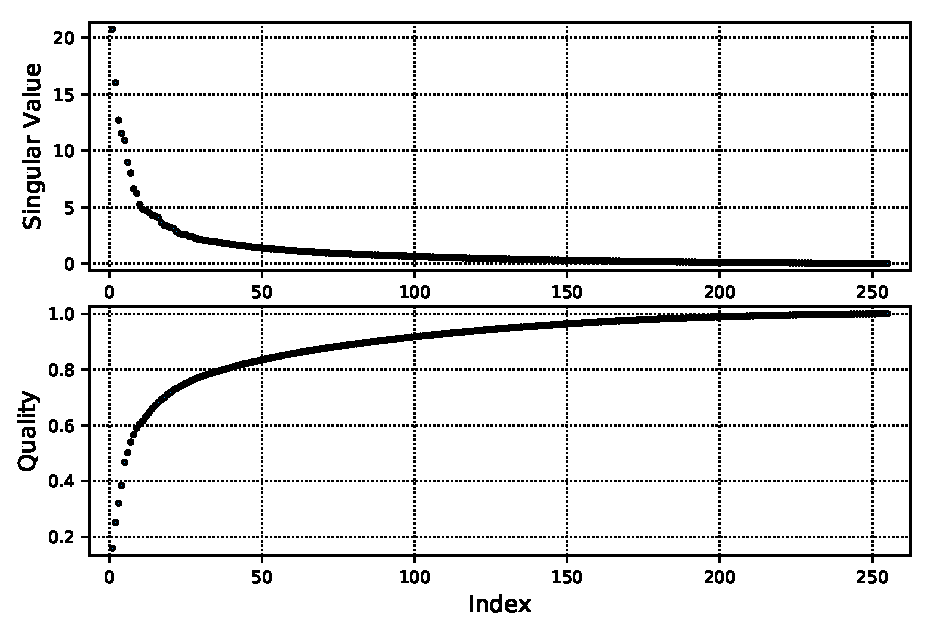
\includegraphics[]{plot}
\caption{Comparing Singular Values and Image Quality (Index $=k$)}\label{fig:singularvalues}
\end{figure}


\pagebreak







\section{Handwritten Digit Classification}

Handwritten digit classification is the following problem: As our \textit{training} data, we are given ten collections of digit images (0 through 9) where each collection contains various images of the same digit.  We are then given an image of an unknown digit from \textit{testing} data (usually disjoint from training data) and are tasked with determining which class this unknown digit most likely belongs to.

The data used was from a subset of the MNIST database found at \cite{mnist}.  This consists of a sample of handwritten digits where each is represented as a $28\times 28$ grayscale image.





\subsection{Overview of the Model}
It is often advantageous to take data in a high dimensional space and represent it in a lower dimension.  This approach mitigates  model over-fitting which allows it to generalize better to new data.  We will use the singular value decomposition and the concepts of low rank approximation developed in the previous section to represent our data in a particular basis that will allow us to best approximate it in a lower dimension.

$$
$$

Consider a $28\times 28$ gray-scale image represented as in the previous section.  Now, take the image matrix and stack the columns in order to produce a vector $v\in \mathbb{R}^{784}$.  This is how a single image will be represented in our model.

To represent an image class $i$, form the matrix $A^{(i)}$ where each column of $A^{(i)}$ is an image vector of a digit from class $i$ in our training set.  Thus, if we have $n$ digits in our training set for class $i$, then $A^{(i)} \in \mathbb{R}^{784\times n}$.

Next, we will use the singular value decomposition and form a reduced rank approximation $A^{(i)}_k = U^{(i)}_k\Sigma_k^{(i)}V^{(i)T}_k$ of $A^{(i)}$.  It will be shown that the columns of $U_k^{(i)}$ form an orthogonal basis for the images in $A^{(i)}$ in the lower $k$ dimension.

Then, classification of a new, unknown digit $z$ is simply the task of finding which image class basis represents $z$ the best.  Viewed in another way, for each digit class we see how well $z$ can be represented as a linear combination of images in that class.


\subsection{Theory Behind the Model}

From this point onwards, when we refer to a matrix $A$ without the superscript $(i)$, it means that $A$ can represent an arbitrary image class.


\begin{theorem}
Let A $\in \mathbb{R}^{m \times n}$ have $\text{rank} (A) = r \leq \min \{m,n\}$ and slim singular value decomposition $A=U_r\Sigma_rV_r^T$. Then
\begin{equation}
\min_x \vecnorm{Ax-b} = V_r\Sigma_r^{-1}U_r^Tb
\end{equation}
\end{theorem}

\textit{Proof.} [See \cite{elden} for proof].


$$
$$

Suppose that $A$ has rank $r$ and we have $k$ such that $k<r$.  Consider the range of $A$, let $x\in \mathbb{R}^n$, then

%$$
%Ax = \sum_{i=1}^r \sigma_i u_i v_i^T x = \sum_{i=1}^r \alpha_i u_i
%\quad
%\text{where $\alpha_i=\sigma_iv_i^Tx$, $\:$ note that both %$\sigma_i$ and $v_i^Tx$ are scalars.}
%$$

$$
Ax \approx A_k x = \sum_{i=1}^k \sigma_i u_i v_i^T x = \sum_{i=1}^k \alpha_i u_i
\quad
\text{where $\alpha_i=\sigma_iv_i^Tx$, $\:$ note that both $\sigma_i$ and $v_i^Tx$ are scalars.}
$$

So the columns of $U_k$ form an orthonormal basis for the range of $A$.  If we have an unknown digit $z\in \mathbb{R}^{m}$, then its representation in the current digit basis is given by $\sum_{i=1}^k\alpha_iu_i$ for some scalars $\alpha_i$.  Therefore, if we wish to find the best representation of this unknown digit in our current digit space, we must solve the  following minimization problem.

\begin{equation}
\min_{\alpha} \vecnorm{z-\sum_{i=1}^k\alpha_iu_i}
= \min_{\alpha} \vecnorm{z-U_k\alpha}
,\:
\text{for $\alpha \in \mathbb{R}^{k}$}
\end{equation}

Since $U_k$ has orthogonal columns, the slim singular value decomposition of $U_k$ is $U_k^T$.  This is because $U_k = XDY$ where $X$ is $U_k$, and $D$ and $Y$ are the $k\times k$ identity matrix ($I$ is diagonal and orthogonal).

Combining the above with equation $(6)$ from the Least Squares theorem we see that in order to minimize $(7)$ we can choose $\alpha = U_k^Tz$.

Doing so results in the minimum value of

\begin{equation}
\min_{\alpha} \vecnorm{z-U_k\alpha} = \vecnorm{z-U_kU_k^Tz} = \vecnorm{(I-U_kU_k^T)z}
\end{equation}

This value is very important in the implementation of the classifier.  For the unknown digit, this value is computed for each image class and the class that minimizes this value is most likely the class that this unknown digit belongs to.


\subsection{Results}

A subset of the MNIST handwritten digit data \cite{mnist} was partitioned randomly into 1000 training images and 1000 test images.  There was approximately an equal distribution of digits from the different classes in both the training and test sets.

$$
$$

Figure $(4)$ shows select vectors from $U^{(3)}$.  We see that the first singular vector $u_1$ resembles the mean of all the 3's in the training set.  Subsequent vectors model variations in the 3's and combine together to form the individual features of the various 3's in the training set.

$$
\text{Optimal accuracy of \textbf{96.2\%} was achieved using a rank $15$ approximation.}
$$

\begin{figure}[H]
\centering
        \begin{subfigure}[b]{0.22\textwidth}
                \centering
                \includegraphics[width=\linewidth]{first3}
                \caption{$u_1$}
                \label{fig:first3}
        \end{subfigure}\hfill
        \begin{subfigure}[b]{0.22\textwidth}
                \centering
                \includegraphics[width=\linewidth]{second3}
                \caption{$u_2$}
                \label{fig:second3}
        \end{subfigure}\hfill
        \begin{subfigure}[b]{0.22\textwidth}
                \centering
                \includegraphics[width=\linewidth]{fourth3}
                \caption{$u_3$}
                \label{fig:fourth3}
        \end{subfigure}\hfill
        \begin{subfigure}[b]{0.22\textwidth}
                \centering
                \includegraphics[width=\linewidth]{tenth3}
                \caption{$u_{15}$}
                \label{fig:tenth3}
        \end{subfigure}
        \caption{Singular Images (Columns of $U$)}\label{fig:components}
\end{figure}



\begin{figure}[H]
\centering
\includegraphics[scale=3]{bad3}
\caption{Digit 3 that was classified as a 5}
\end{figure}


\begin{figure}[H]
\centering
\includegraphics[scale=0.5]{rankAccuracy}
\caption{Rank Reduced Approximation Results}
\end{figure}

This approach was easy to implement, at most requiring functionality to find the SVD of a matrix.  These calculations are relatively quick and once the basis matrices are calculated for each digit class, the actual classification only requires matrix multiplication.  An interesting strength of this model is its ability to extend itself easily to include more classes.  Suppose that you wanted to add another character for classification and obtained training data for this character.  In contrast to other models such as neural networks which would require time consuming retraining, adding another class to this approach only requires the computation of one more SVD.


\section{Conclusion}

It was shown how the SVD of a matrix produces an intuitive approximation for the original matrix, and the Eckart-Young Theorem was presented that proved that this approximation is in fact optimal.  This approach was directly applied to image compression, and was also demonstrated in the construction of a reduced rank model for image classification.

\section{Project Code}

The code used to generate the results of this project was written in Julia 0.5.1, the major sections are listed below.

\begin{algorithm}
\caption{Image Compression}

\begin{lstlisting}
using Images, TestImages, Interact

function compress_gray(img, rank)
    range = 1:rank
    U,S,V = svd(img)
    return Gray.(U[:,range] * Diagonal(S[range]) * V[:,range]')
end

function compress_colour(img, rank)
    channels = float(channelview(img))
    redApprox = compress_gray(channels[1,:,:], rank)
    greenApprox = compress_gray(channels[2,:,:], rank)
    blueApprox = compress_gray(channels[3,:,:], rank)
    
    return colorview(RGB, redApprox, greenApprox, blueApprox)
end
\end{lstlisting}

\end{algorithm}



\begin{algorithm}
\caption{Obtain MNIST data from LIBSVM format}

\begin{lstlisting}
using Images, Colors

type Digit
    label::Integer
    vector::Array{Float64,1}
end

function parse_LIBSVM(line::String, size::Int) 
    vector = zeros(size)
    split_line = split(line)

    label = parse(Int, split_line[1])

    for entry in split_line[2:end]
        split_entry = parse.(split(entry,":"))
        vector[split_entry[1]] = split_entry[2]
    end
    
    return Digit(label,vector)
end

function get_data(filename::String)

    size = 784

    digit_classes = [Array{Float64}(size,0) for dim in 1:10]

    for line in readlines(open(filename))
        result = parse_LIBSVM(line,size)
        label = result.label
        if label == 0
            label = 10
        end

        vector = result.vector
        # center the data for classification
        vector -= mean(vector)

        # append the digit to its class collection
        digit_classes[label] = hcat(digit_classes[label],vector)

    end
    
    return digit_classes
end
\end{lstlisting}

\end{algorithm}


\begin{algorithm}
\caption{Classification}

\begin{lstlisting}
function get_SVDs(digit_classes)

    U_collection, S_collection, V_collection = [],[],[]

    for A in digit_classes
        U, S, V = svd(A)
        push!(U_collection,U)
        push!(S_collection,S)
        push!(V_collection,V)
    end

    return U_collection, S_collection, V_collection
end

function classification_residual(vector, digit_class, k, U_collection)
    Uk = U_collection[digit_class][:,1:k]
    closest = (eye(784) - Uk*Uk')*vector
    return norm(closest, 2)
end

function classification_residuals(vector, k, U_collection)
    return [classification_residual(vector, digit_class, k, U_collection) for digit_class in 1:10]
end

function predict_class(residuals)
    class_index = find(x->x==minimum(residuals), residuals)[1]
    if class_index == 10
        class_index = 0
    end
    return class_index
end

function classification_results(unknown_digits, U_collection, k)
    
    correct = 0
    incorrect = 0

    for class_index in 1:10
        println("k: $k")
        println(class_index)
        unknown_digit_collection = unknown_digits[class_index]
        for unknown_digit_col in 1:size(unknown_digit_collection)[2]

            unknown_digit = unknown_digit_collection[:,unknown_digit_col]
            predicted_index = predict_class(classification_residuals(unknown_digit, k, U_collection))

            correct += predicted_index == (class_index%10)
            incorrect += predicted_index != (class_index%10)
        end
    end

    return correct,incorrect
    
end
\end{lstlisting}

\end{algorithm}


\begin{algorithm}
\caption{Display Digits}

\begin{lstlisting}
function display_digit(digit_matrix, col)
    Gray.(1-reshape(digit_matrix[:,col],(28,28))')
end

function display_singular_vector(vec)
    result = reshape(vec, (28,28))
    result -= minimum(vec)
    result /= maximum(result)

    return Gray.(1-result)'
end
\end{lstlisting}

\end{algorithm}

\bibliographystyle{alpha}
\bibliography{sample}



\end{document}